%%% The main file. It contains definitions of basic parameters and includes all other parts.

% Meta-data of your thesis (please edit)
\input metadata.tex

% Generate metadata in XMP format for use by the pdfx package
\input xmp.tex

%% Settings for single-side (simplex) printing
% Margins: left 40mm, right 25mm, top and bottom 25mm
% (but beware, LaTeX adds 1in implicitly)
\documentclass[12pt,a4paper]{report}
\setlength\textwidth{145mm}
\setlength\textheight{247mm}
\setlength\oddsidemargin{15mm}
\setlength\evensidemargin{15mm}
\setlength\topmargin{0mm}
\setlength\headsep{0mm}
\setlength\headheight{0mm}
% \openright makes the following text appear on a right-hand page
\let\openright=\clearpage

%% Settings for two-sided (duplex) printing
% \documentclass[12pt,a4paper,twoside,openright]{report}
% \setlength\textwidth{145mm}
% \setlength\textheight{247mm}
% \setlength\oddsidemargin{14.2mm}
% \setlength\evensidemargin{0mm}
% \setlength\topmargin{0mm}
% \setlength\headsep{0mm}
% \setlength\headheight{0mm}
% \let\openright=\cleardoublepage

%% If the thesis has no printed version, symmetric margins look better
% \documentclass[12pt,a4paper]{report}
% \setlength\textwidth{145mm}
% \setlength\textheight{247mm}
% \setlength\oddsidemargin{10mm}
% \setlength\evensidemargin{10mm}
% \setlength\topmargin{0mm}
% \setlength\headsep{0mm}
% \setlength\headheight{0mm}
% \let\openright=\clearpage

%% Generate PDF/A-2u
\usepackage[a-2u]{pdfx}

%% Prefer Latin Modern fonts
\usepackage{lmodern}
% If we are not using LuaTeX, we need to set up character encoding:
\usepackage{iftex}
\ifpdftex
\usepackage[utf8]{inputenc}
\usepackage[T1]{fontenc}
\usepackage{textcomp}
\fi

%% Further useful packages (included in most LaTeX distributions)
\usepackage{amsmath}        % extensions for typesetting of math
\usepackage{amsfonts}       % math fonts
\usepackage{amsthm}         % theorems, definitions, etc.
\usepackage{bm}             % boldface symbols (\bm)
\usepackage{booktabs}       % improved horizontal lines in tables
\usepackage{caption}        % custom captions of floating objects
\usepackage{dcolumn}        % improved alignment of table columns
\usepackage{floatrow}       % custom float environments
\usepackage{graphicx}       % embedding of pictures
\usepackage{indentfirst}    % indent the first paragraph of a chapter
\usepackage[nopatch=item]{microtype}   % micro-typographic refinement
\usepackage{paralist}       % improved enumerate and itemize
\usepackage[nottoc]{tocbibind} % makes sure that bibliography and the lists
			    % of figures/tables are included in the table
			    % of contents
\usepackage{xcolor}         % typesetting in color

% The hyperref package for clickable links in PDF and also for storing
% metadata to PDF (including the table of contents).
% Most settings are pre-set by the pdfx package.
\hypersetup{unicode}
\hypersetup{breaklinks=true}

% Packages for computer science theses
\usepackage{algpseudocode}  % part of algorithmicx package
\usepackage{algorithm}
\usepackage{fancyvrb}       % improved verbatim environment
\usepackage{listings}       % pretty-printer of source code

% You might want to use cleveref for references
% \usepackage{cleveref}

% Set up formatting of bibliography (references to literature)
% Details can be adjusted in macros.tex.
%
% BEWARE: Different fields of research and different university departments
% have their own customs regarding bibliography. Consult the bibliography
% format with your supervisor.
%
% The basic format according to the ISO 690 standard with numbered references
\usepackage[natbib,style=iso-numeric,sorting=none]{biblatex}
% ISO 690 with alphanumeric references (abbreviations of authors' names)
%\usepackage[natbib,style=iso-alphabetic]{biblatex}
% ISO 690 with references Author (year)
%\usepackage[natbib,style=iso-authoryear]{biblatex}
%
% Some fields of research prefer a simple format with numbered references
% (sorting=none tells that bibliography should be listed in citation order)
%\usepackage[natbib,style=numeric,sorting=none]{biblatex}
% Numbered references, but [1,2,3,4,5] is compressed to [1-5]
%\usepackage[natbib,style=numeric-comp,sorting=none]{biblatex}
% A simple format with alphanumeric references:
%\usepackage[natbib,style=alphabetic]{biblatex}

% Load the file with bibliography entries
\addbibresource{bibliography.bib}

% Our definitions of macros (see description inside)
\input macros.tex

%%% Title page and various mandatory informational pages
\begin{document}
%%% Title page of the thesis and other mandatory pages

%%% Inscriptions at the opening page of the hard cover

% We usually do not typeset the hard cover, but if you want to do it, change \iffalse to \iftrue
\iffalse

\pagestyle{empty}
\hypersetup{pageanchor=false}
\begin{center}

\large
Charles University

\medskip

Faculty of Mathematics and Physics

\vfill

{\huge\bf\ThesisTypeTitle}

\vfill

{\huge\bf\ThesisTitle\par}

\vfill
\vfill

\hbox to \hsize{\YearSubmitted\hfil \ThesisAuthor}

\end{center}

\newpage\openright
\setcounter{page}{1}

\fi

%%% Title page of the thesis

\pagestyle{empty}
\hypersetup{pageanchor=false}
\begin{center}

\centerline{\mbox{
\includegraphics[width=166mm]{img/logo-en.pdf}}}

\vspace{-8mm}
\vfill

{\bf\Large\ThesisTypeTitle}

\vfill

{\LARGE\ThesisAuthor}

\vspace{15mm}

{\LARGE\bfseries\ThesisTitle\par}

\vfill

\Department

\vfill

{
\centerline{\vbox{\halign{\hbox to 0.45\hsize{\hfil #}&\hskip 0.5em\parbox[t]{0.45\hsize}{\raggedright #}\cr
Supervisor of the \ThesisTypeName{} thesis:&\Supervisor \cr
\ifx\ThesisType\TypeRig\else
\noalign{\vspace{2mm}}
Study programme:&\StudyProgramme \cr
\fi
}}}}

\vfill

Prague \YearSubmitted

\end{center}

\newpage

%%% A page with a solemn declaration to the thesis

\openright
\hypersetup{pageanchor=true}
\vglue 0pt plus 1fill

\noindent
I declare that I carried out this \ThesisTypeName{} thesis on my own, and only with the cited
sources, literature and other professional sources.
I understand that my work relates to the rights and obligations under the Act No.~121/2000 Sb.,
the Copyright Act, as amended, in particular the fact that the Charles
University has the right to conclude a license agreement on the use of this
work as a school work pursuant to Section 60 subsection 1 of the Copyright~Act.

\vspace{10mm}

\hbox{\hbox to 0.5\hsize{%
In \hbox to 6em{\dotfill} date \hbox to 6em{\dotfill}
\hss}\hbox to 0.5\hsize{\dotfill\quad}}
\smallskip
\hbox{\hbox to 0.5\hsize{}\hbox to 0.5\hsize{\hfil Author's signature\hfil}}

\vspace{20mm}
\newpage

%%% Dedication

\openright

\noindent
\Dedication

\newpage

%%% Mandatory information page of the thesis

\openright
{\InfoPageFont

\vtop to 0.5\vsize{
\setlength\parindent{0mm}
\setlength\parskip{5mm}

Title:
\ThesisTitle

Author:
\ThesisAuthor

\DeptType:
\Department

Supervisor:
\Supervisor, \SupervisorsDepartment

Abstract:
\Abstract

Keywords:
{\def\sep{\unskip, }\ThesisKeywords}

\vfil
}

% In Czech study programmes, it is mandatory to include Czech meta-data:

\ifx\StudyLanguage\LangCS

\vtop to 0.49\vsize{
\setlength\parindent{0mm}
\setlength\parskip{5mm}

Název práce:
\ThesisTitleCS

Autor:
\ThesisAuthor

\DeptTypeCS:
\DepartmentCS

Vedoucí bakalářské práce:
\Supervisor, \SupervisorsDepartmentCS

Abstrakt:
\AbstractCS

Klíčová slova:
{\def\sep{\unskip, }\ThesisKeywordsCS}

\vfil
}

\fi

}

\newpage

%%% Further pages will be numbered, which LaTeX automatically enables at the next chapter start


%%% A page with automatically generated table of contents of the thesis

\tableofcontents

%%% Each chapter is kept in a separate file
\chapter*{Introduction}
\addcontentsline{toc}{chapter}{Introduction}



\ldots
\textbf{The goal of this thesis is to explore the possibility to explore the possibility}

\chapter{Abstract Interpretation}

\xxx{TODO add some more introduction (or it will probably be in the Introduction part)?}

In this chapter, we will build the theory of Abstract Interpretation from scratch, so that we are able to use the method
for the analysis in the future chapters.
We will start by defining what we mean by a Program and what can be considered an approximation of a Program.
In order to understand Abstract Interpretation, we will next dive into the theory of algebraic structure called Lattice.
Then, with all we will have done, we will be able to define Galois connection - the essence of the method itself.

\section{Program and approximation}

\subsection{Syntax}

We define a simple language: % TODO comment?

\begin{defn}[Expression]
    Expresion is defined inductively:
    \begin{itemize}
        \item a constant $n \in \mathbb{Z}$ is an expression
        \item a variable $x$ is an expression
        \item for each pair $E$, $F$ of expressions the following are also expressions: $E+F$, $E-F$, $E * F$, $E/F$, $E \geq F$
    \end{itemize}
\end{defn}

\begin{defn}[Statement] % TODO or Command?
    The following are statements:
    \begin{itemize}
        \item exit
        \item $x = E$ for expression $E$ %todo format
        \item if $E$ goto $n$ for expression $E$ and constant $n$
        \item input x
        \item output E for expression $E$
    \end{itemize}
    We will denote the set of all statements $\mathbb{S}$
\end{defn}

\subsection{Semantic}

\begin{defn}[Program]
    Program is a function $P: \mathbb{Z} \rightarrow \mathbb{S}$
\end{defn}

\begin{defn}[Trace]
\end{defn}[Trace]

\subsection{Approximation}



\section{Lattices}

The Abstract Interpretation is defined on Lattices - algebraic structures with additional ordering constraints.
In this subchapter, we will cover

\begin{defn}[Partially ordered set]
    Partially ordered set is a tuple $(M, \leq)$, where $M$ is a (possibly infinite) set and $\leq$ is a binary relation
    which is:
    \begin{itemize}
        \item Reflexive: $\forall x \in M, x \leq x$
        \item Antisymmetric: $\forall x, y \in M, a \leq b \land b \leq a \implies a = b$
        \item Transitive: $\forall x, y, z \in M, x \leq y \land y \leq z \implies x \leq z$
    \end{itemize}
\end{defn}



\section{Galois connections, abstraction and concretization} % TODO shorter name

\chapter{Data manipulation and Pandas library}

In this chapter, our goal is to explore the world of data manipulation.
We explain what data structures are usually used and what the common operations on them look like.
We will need the information in the next chapters when defining the Abstract Interpretation framework for these data
structures.
We show the concepts on Pandas and discuss what Pandas does differently.

\section{Data structures} %============================================================================================%

When we talk about data structure, we usually define it as a way of organizing data in the computer memory.
However, there are two concepts to distinguish---the interface and the implementation.

The interface is a set of operations that we are allowed to do with the data structure as users.
A Good example of a data structure interface can be an Array, List, Dictionary or a Heap.
Implementation on the other hand is how the data structure works under the hood to provide the interface promised.
To give an example of an implementation of a data structure, I mention a binary tree, n-ary heap or a linked list.

In this chapter, when talking about data structures, we omit the implementation details, and we focus only on the
interface of the data structure, i.e.,~what operations are provided.
Also, we assume the existence of primitive data types such as integers, floating-point numbers, strings etc.

\begin{defn}[List interface]
    \textbf{List} interface is a set of methods for random access, appending, inserting, updating and removing elements
    from a collection.
    All operations use numeric zero-based indexing.
\end{defn}

\begin{defn}[Dictionary interface]
    \textbf{Dictionary} interface supports accessing, adding, replacing or removing elements from a collection.
    All operations use key-based indexing.
\end{defn}

\subsection{Series}

The first and the simplest data structure is usually called Series.
In its simplest form, it is a one-dimensional data structure that holds data of some primitive data type.
It supports a List interface, so random access based on integer indexing is supported as well as adding, removing and
modifying items.

The Listing~\ref{lst:series_basics} shows basic work with the Series data structure in Pandas.

\begin{lstlisting}[caption=Working with Series in Pandas, label={lst:series_basics}, captionpos=b]
import pandas as pd
# Creating Series
series = pd.Series([1, 1, 2, 3, 5, 8])

# Adding an element
series[6] = 13

# Removing an element at index 0
series.drop(0, inplace=True)

# Replacing an element
series[1] = 100
\end{lstlisting}

There can also be an index associated with the Series.
The index is a set of distinct values of any primitive type (usually a string or a time) associated with the values of
the Series.
It expands the interface of a Series with a Dictionary interface.
Consequently, the items can be accessed using the values in the index.
Another usual feature of a Series is an optional label describing the data.
Listing~\ref{lst:series_index} shows how the work with index works in Pandas.

\begin{lstlisting}[caption=Index on a Series, label={lst:series_index}, captionpos=b]
import pandas as pd

# Creating Series with index
data = [1, 2, 3, 4]
index = ["first", "second", "third", "fourth"]
series = pd.Series(data=data, index=index)

# Accessing based on index
print(series["second"]) # Prints 2

# Adding based on index
series["fifth"] = 5

# Removing based on index
series.drop("fifth", inplace=True)

\end{lstlisting}

Contrary to what we said, Series in Pandas is a heterogeneous data structure---it is able to hold values of different
types together.
So the code showed in Listing~\ref{lst:series_heterogeneous} is completely valid Pandas code.

\begin{lstlisting}[caption=Heterogenous Series, label={lst:series_heterogeneous}, captionpos=b]
import pandas as pd

# Create a Series of values with different types
series = pd.Series([0, True, "two", "three", 4])
\end{lstlisting}

The explanatory visualization of a Series can be found in the Figure~\ref{fig:series_schema}

\begin{figure}[H]
    \caption{Schema of a Series}
    \label{fig:series_schema}
    \centering
    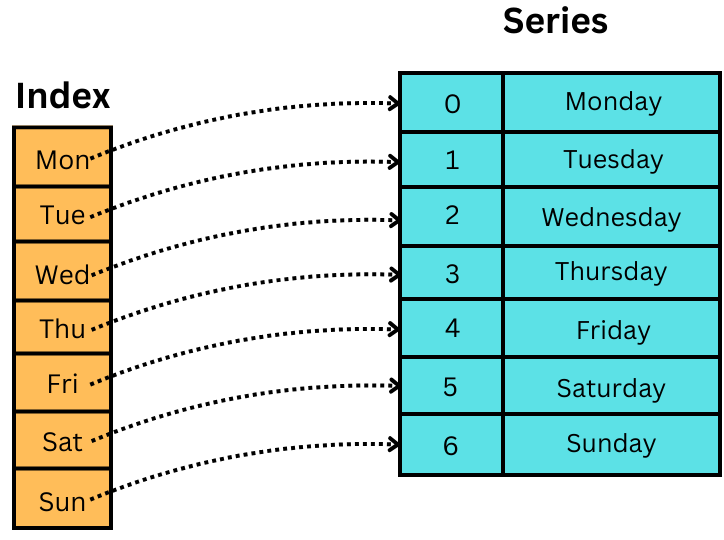
\includegraphics[scale=0.4]{img/Series}
\end{figure}

\subsection{Dataframe}

Dataframe is a two-dimensional tabular data structure.
A good way to look at a Dataframe is to see it as a Dictionary, where the keys are names of the columns of a table
and values are Series representing the columns themselves.
This also means that the Dataframe supports indexing of columns based on column names and integer-based indexing of rows.
Listing~\ref{lst:dataframe_basics} shows basic work with the Dataframe in Pandas.

\begin{lstlisting}[caption=Working with Dataframe in Pandas, label={lst:dataframe_basics}, captionpos=b]
import pandas as pd

# Create a Dataframe from a map of columns
data = {"column1": [1, 2, 3], "column2": ['a', 'b', 'c']}
dataframe = pd.DataFrame(data)

# Add a new row
dataframe.loc[3] = [4, 'd']

# Add a new column
dataframe['column3'] = [True, False, True, False]

# Replace a value
dataframe.at[1, 'column3'] = True
\end{lstlisting}

The Dataframe can also have an index associated with the rows of Series.
Consequently, the Dataframe supports Dictionary interface on both rows and columns.
Adding of new columns and rows is also supported.
The listing~\ref{lst:dataframe_index} shows how we can use indexes when working with Dataframes in Pandas.

\begin{lstlisting}[caption=Index on a Dataframe, label={lst:dataframe_index}, captionpos=b]
import pandas as pd

# Create a dataframe with index
dataframe = pd.DataFrame({
    'A': [1, 2, 3],
    'B': [4, 5, 6],
    'C': [7, 8, 9]
}, index=['x', 'y', 'z'])

# Access elements via index
print(dataframe.at['x', 'A']) # Prints 1

# Change value using index
dataframe.at['z', 'C'] = -9
\end{lstlisting}

The explanatory visualization of a Dataframe can be found in the Figure~\ref{fig:dataframe_schema}

\begin{figure}[H]
    \caption{Schema of a Dataframe}
    \label{fig:dataframe_schema}
    \centering
    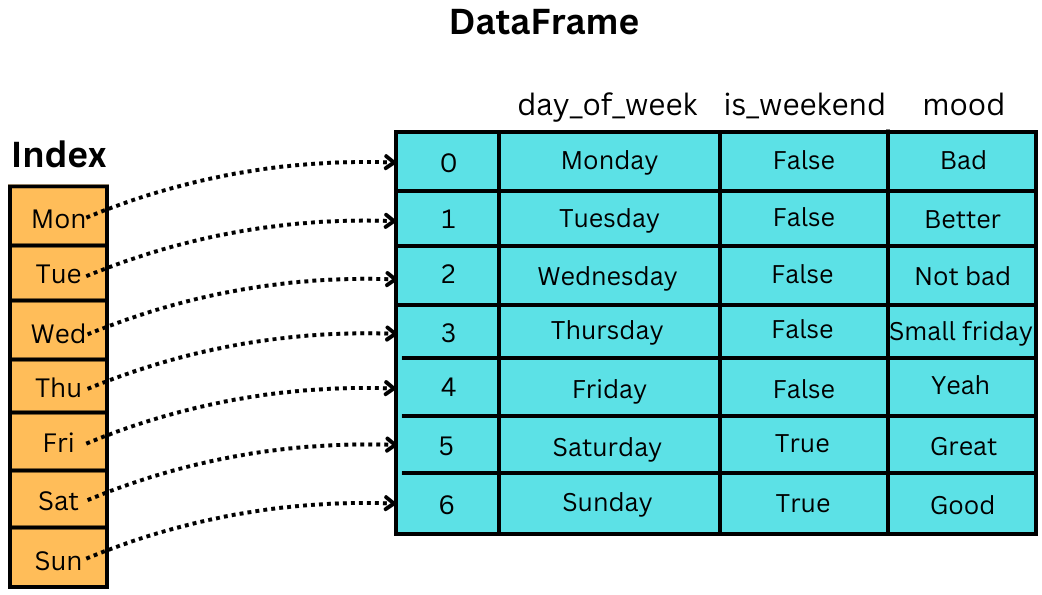
\includegraphics[scale=0.4]{img/Dataframe}
\end{figure}

The Dataframe is usually loaded from a CSV file via the \verb|read_csv| function, and the Dataframe that is the result
of the computation is usually stored to another CSV file via the \verb|to_csv| function.


\section{Common operations} %==========================================================================================%

To actually manipulate the data into some useful form, we need operations that are more powerful than just indexing and
adding and removing elements.
The operations that are commonly used in data manipulation were greatly influenced by the operations on relational
databases and the SQL language.
However, they are usually more flexible and customizable.

\subsection{Relational operations}

All well-known SQL relational databases support the following operations:
\texttt{SELECT, GROUP BY, HAVING, WHERE, JOIN, ORDER BY, AS}.
\\All these operations are also (usually under a different name) present in the data manipulation libraries as well.
We go through these operations and discuss their counterparts in Pandas.

\paragraph{SELECT} \leavevmode \\

The SELECT statement in SQL serves to select a specific subset of columns of a table.
In Pandas the square-brackets operator is used for that purpose.
As listing~\ref{lst:pandas_select} shows, the operator can return a Series or a Dataframe depending on whether
the argument is just a string or a list of strings.

\begin{lstlisting}[caption=Select in Pandas, label={lst:pandas_select}, captionpos=b]
dataframe = ... # initial dataframe

# Select a subset of columns (returns a dataframe)
subset = dataframe[["column1", "column3"]]

# Select one column (returns a Series)
column = dataframe["column2"]
\end{lstlisting}

Alternatively, the filter function can be also used for this purpose.
The important information for us will be that the operation returns a Dataframe with a different column structure
than the input Dataframe---it removes non-specified columns.

The SELECT statement in SQL can also do more than just selecting a subset of columns.
It can also apply aggregating function when used with group by.
This option is covered later when we talk about the GROUP BY operation.

\paragraph{WHERE} \leavevmode \\

The WHERE statement in SQL filters out the rows that do not match a given predicate.
In this case, Pandas was also able to make use of the square-brackets operator.
This time the operator accepts a Series of bool values and uses just the columns of a Dataframe with index the same as
some True value in the Series.
The Series of bools is usually (but not necessarily) created using vectorized operations.
The listing~\ref{lst:pandas_where} shows the usage.

\begin{lstlisting}[caption=Where in Pandas, label={lst:pandas_where}, captionpos=b]
dataframe = ... # initial dataframe

# Select just rows where the "age" column is at least 18
adults = dataframe[dataframe["age"] >= 18]
\end{lstlisting}

The important information for us will be that the result of this operation is a Dataframe with the same column structure.

\paragraph{AS} \leavevmode \\

The AS keyword is used to rename a specific column.
Pandas also has this feature, although it is named differently.
The function is called rename, and it accepts a mapping from old column names to new column names.
The listing~\ref{lst:pandas_as} shows how the rename function can be used.

\begin{lstlisting}[caption=As in Pandas, label={lst:pandas_as}, captionpos=b]
dataframe = ... # initial dataframe

# Rename some of the columns
renamed_dataframe = dataframe.rename(
    columns={"column1": "col1", "column2": "col2"}
)
\end{lstlisting}

\paragraph{ORDER BY} \leavevmode \\

ORDER BY is used to sort the data by some columns.
Pandas can do the same using the sort\_values function.
The example usage can be seen in the listing~\ref{lst:pandas_orderby}

\begin{lstlisting}[caption=Order by in Pandas, label={lst:pandas_orderby}, captionpos=b]
dataframe = ... # initial dataframe

# Order the dataframe rows by the values of column
# 'surname' in the ascending order
sorted = dataframe.sort_values(by=["surname"], ascending=True)
\end{lstlisting}

Note that the operation does not change the column structure of the Dataframe.

\paragraph{JOIN} \leavevmode \\

Join operation is used to combine rows from two tables based on some related columns.
There are four types of join---inner, left, right and outer.
Inner join returns rows that have matching rows in both tables.
Left join returns all rows from the left table and all matched rows from the right table.
Right join returns all rows from the right table and all matched rows from the left table.
And outer join returns rows where there is a match in either of the tables.

Pandas has a function called merge for this purpose.
It accepts two Dataframes and returns their corresponding join.
Besides the already mentioned joins, merge also supports a cross-join, which is essentially a cartesian product of
two sets of rows.
The listing~\ref{lst:pandas_join} shows how the merge function can be used as well as what parameters does the
function accept.

\begin{lstlisting}[caption=Join in Pandas, label={lst:pandas_join}, captionpos=b]
dataframe1 = ... # 1st initial dataframe
dataframe2 = ... # 2nd initial dataframe

inner = pd.merge(
    dataframe1, dataframe2, how="inner",
    left_on="left_key", right_on="right_key")
left = pd.merge(
    dataframe1, dataframe2, how="left", on="common_key")
right = pd.merge(
    dataframe1, dataframe2, how="right", on="common_key")
outer = pd.merge(
    dataframe1, dataframe2, how="outer",
    left_on="left_key", right_on="right_key"
cross = pd.merge(
    dataframe1, dataframe2, how="cross")
\end{lstlisting}

\paragraph{GROUP BY} \leavevmode \\

The group by operation aggregates the rows based on specified columns.
It does not return normal rows but summary rows, which we can apply aggregate functions on.
A Good example of an aggregate function can be max, min or sum.

Pandas has a function with the same name---groupby.
The function returns a DataframeGroupBy object, which we can apply aggregate functions on.
The listing~\ref{lst:pandas_groupby} shows the usage

\begin{lstlisting}[caption=Group by in Pandas, label={lst:pandas_groupby}, captionpos=b]
dataframe = ... # initial dataframe

# Group the dataframe by agg_column and return
# the mean of the "salary" column
dataframe.groupby(by=["work_department"])["salary"].mean()
\end{lstlisting}

\paragraph{HAVING} \leavevmode \\

Having operation works somewhat like a where operation on a summary rows---where group by was already applied.
In having clause, we can use any aggregate function in a predicate and then filter the summary rows based on such
predicate.

In Pandas, this can be done in many ways, but the usual one involves the filter function and lambdas.
Example of such usage is shown in the listing~\ref{lst:pandas_having}.

\begin{lstlisting}[caption=Having in Pandas, label={lst:pandas_having}, captionpos=b]
dataframe = ... # initial dataframe

# Group the dataframe by agg_column and return
# the columns that are in a work_department
# with an average salary higher than 10 000
dataframe \
    .groupby(by=["work_department"]) \
    .filter(lambda x: x["salary"].mean() > 10000)
\end{lstlisting}


\subsection{Vectorized operations}

When we discussed the SQL WHERE clause, we came across the following line of code:

\verb|adults = dataframe[dataframe["age"] >= 18]|

We said that this line of code filters out the rows where the age is less than 18.
We also said that the square-bracket operator accepts a Series of bools.
So the expression~\verb|dataframe["age"] >= 18]| must return a Series of bools.
But why does this work?
How can we compare a Series to a number?

In Pandas, the Series can be summed, subtracted, multiplied or compared with values that are either Series or a scalar
values.
The listing~\ref{lst:vectorized_operations} shows the behavior of some vectorized operations in Pandas performed in
the interactive mode.

\begin{lstlisting}[caption=Vectorized operations, label={lst:vectorized_operations}, captionpos=b]
>>> sr1 = pd.Series([1, 2, 3])
>>> sr1 + 7
0     8
1     9
2    10
dtype: int64
>>> 3 * sr1
0    3
1    6
2    9
dtype: int64
>>> sr1 / sr1
0    1.0
1    1.0
2    1.0
dtype: float64
>>> sr2 = pd.Series(["a", "b", "c"])
>>> sr2 * 2
0    aa
1    bb
2    cc
dtype: object
>>> sr2 + "x"
0    ax
1    bx
2    cx
dtype: object
\end{lstlisting}

\section*{Summary} %===================================================================================================%
\addcontentsline{toc}{section}{Summary}

We covered two common data structure interfaces used in data analysis - Series and Dataframe.
Series is a one-dimensional List-like data structure with support for index and an axis label.
Data frame is a two-dimensional structure---a dictionary of columns.
The whole Dataframe can have an index associated, and the column of a Dataframe can be seen as a Series.
Many operations in the data manipulation libraries are influenced by the SQL language operations such as join, select,
group by, where, order by etc.
The data structures also support vectorized operations like sums, products or comparing.

All discussed topics were demonstrated on Pandas code snippets.
However, the Pandas library is a large project and the goal of this chapter was not to explore it all.
More detailed information can be found in the API reference of Pandas\cite{pandas_docs}.

\chapter{Putting it all together}\label{ch:putting-it-all-together}

As the name of this chapter suggests, we now put the knowledge from the previous chapters together.
We build the Abstract Interpretation framework for data manipulation programs.
It involves defining the concrete and abstract lattice and the Galois connection between.

Since we are mostly focusing on Pandas in Python, we assume Python environment with Pandas, specifically:

\begin{itemize}
    \item Python syntax
    \item Standard Python data types - int, float, string, list, dictionary, tuple
    \item Pandas is imported via \verb|import pandas as pd| statement
\end{itemize}

We also assume, unlike the Pandas, that Series are homogenous and Dataframes have homogenous columns.
This also implies that each column of a Dataframe has an associated type.

\begin{defn}
    Let Df be a Dataframe and Sr a Series.
    We assume the following operations for accessing metadata about the two structures:

    \verb|columns(Df) = { Sr1 .. Srn }| \\

    \verb|type(Sr) - returns type| \\

    \verb|name(Sr) - returns name| \\
\end{defn}

Given these assumptions, we can define a Dataframe Structure:

\begin{defn}[Dataframe Structure]
    For a Dataframe $Df$, its \textbf{Dataframe} Structure is $DS(Df) = \{ (name(Sr), type(Sr)) | Sr \in columns(Df) \}$
\end{defn}

Also, we define a Series Structure:

\begin{defn}[Series Structure]
    For a Series $Sr$, its \textbf{Series Structure} is $SS(Sr) = (name(Sr), type(Sr))$
\end{defn}


\section{The concrete lattice}

The concrete lattice should correspond with the reality.
Since the variables of our program are Dataframes and Series, we can imagine the set of all possible Dataframes and
Series (with every finite number of rows/columns and all possible values).
Then we define the concrete lattice as the power set of this set with the inclusion being the ordering. % todo chaotic
To formalize this:

\begin{defn}[The concrete lattice]

    Let
    \begin{gather*}
        C = \{\forall df \: Dataframe: df\} \cup \{\forall sr \: Series: sr\}
    \end{gather*}
    Then the concrete lattice is $L_c = (\powerset{C}, \subseteq)$
\end{defn}


\section{The abstract lattice}

The abstract lattice can be chosen by us depending on how much we want to abstract the values.
We would like the abstraction to be actually useful in practice.
What does this mean?
In the Abstract Interpretation, whenever we should get a value from the user, we approximate it by the supremum of our
lattice.
This is usually done when we do not know anything about the input, since it is the most precise approximation that is
still sound.
However, we can do something smarter.
We will create and use the assumption that whenever the user inputs a Dataframe, the Column Structure of that Dataframe
is known in advance.
This is not a very strong assumption in practice given the fact that the structure of the dataframe is usually known
during the process of writing the program anyway - otherwise we would not be able to write the program at all.

So the abstract lattice consists of the Dataframe Structures and Series Structures.
We take the set of all possible Dataframe Structures and Series Structures.
Then the abstract lattice is the power set of that set with the inclusion being the ordering.
We again formalize this:

\begin{defn}[The abstract lattice]

    Let
    \[A = \{\forall df\: Dataframe: DS(df)\} \cup \{\forall sr \: Series: SS(sr)\}\].
    Then the abstract lattice is $L_a = (\powerset{A}, \subseteq)$
\end{defn}

\section{The Galois Connection}

To create a Galois Connection we need an abstraction function and a concretization function.

In the abstraction function, we start with a set of Dataframes and Series, and we want a set of Dataframe Structures and
Series Structures.
The most natural way to define such function is to take the set of Dataframe Structures (Series Structures) of the
Dataframes (Series) from the input.
Formally:

\begin{defn}[Abstraction function]
    Given the concrete lattice $L_c$
    \begin{gather*}
        \forall X \in L_c \\
        X_{df} = \{df \in X: \: df \: is \: Dataframe\} \\
        X_{sr} = \{sr \in X: \: sr \: is \: Series\} \\
        \alpha(X) = \{DS(df) \forall df \in X_{df}\} \cup \{SS(sr) \forall sr \in X_{sr})\}
    \end{gather*}
\end{defn}

Then we need the Concretization function.
We will define it analogously.
We have a set of Dataframe Structures and Series Structures on the input and want a set of Dataframes and Series
on the output.
So we just take all possible Dataframes (Series) with the given Dataframe (Series) Structure.

\begin{defn}[Concretization function]
    Given the abstract lattice $L_a$
    \begin{gather*}
        \forall X \in L_a \\
        X_{df} = \{df \in X: \: df \: is \: Dataframe Structure\} \\
        X_{sr} = \{sr \in X: \: sr \: is \: Series Structure\} \\
        \alpha(X) =
        \bigcup_{dfs \in X_{df}}  \{df: df \: is \: Dataframe \land DS(df) = dfs\}
        \cup \\
        \bigcup_{srs \in X_{sr}} \{sr: sr \: is \: Series \land SS(sr) = srs\}
    \end{gather*}
\end{defn}

\xxx{TODO prove that this is a galois connection}

\section{Abstract Operations}

In the first chapter we mentioned that the abstract semantics can be systematically derived from the galois connection
and the concrete semantics.
However, it is often not the best way to get to the abstract semantics.
We follow an alternative approach.
We define the operations ourselves, since it is a very intuitive process.
We do not define all the operations that we introduced in the previous chapter, we take a subset of them and
the rest can be found in the Pandalyzer implementation and their formal model can be defined in a similar way as the
operations discussed in this section.

We also define the operations on the single Dataframe (Series) Structures rather than on the sets, since it is
easier to understand.
It can then be extended to the variants with sets in a straightforward way.

\begin{itemize}
    \item SELECT

    The first operation we will abstract is a simple SELECT\@.
    We are abstracting selection of a subset of columns given their names.
    This is easy: We take our Dataframe Structure and remove all columns that do not have the names in the selection.
    \begin{example}

        Input: DataFrameStructure(column1: int, column2, string, column3: bool), select([column1, column3])

        Output: DataFrameStructure(column1: int, column3: bool)
    \end{example}
    In a real analysis we should check that all column name specified in select exist in the DataFrameStructure and
    announce an error if the opposite is true.

    \item WHERE

    The WHERE operation has the nice property that it does not change the Dataframe Structure.
    So we just return the input DataframeStructure.
    In a real analysis we should also check that the column referenced in the predicate exists in the DataFrameStructure
    and the comparison happens between compatible types - we should probably announce an error if we are trying to compare
    a number to a string.

    \item JOIN (merge)

    The JOIN is more interesting.
    The input is two DataframeStructures, type of join and related column names.
    The output should be the DataframeStructure of the joined Dataframe.

    \item GROUP BY \xxx{TODO}



    \item \xxx{TODO add some vectorized operations too}


\end{itemize}

\section{Adding other types}

So far, our framework only works with the Dataframe and Series types.
Usually, however, these are not the only types in our program.
Additionally, there are operations that accept Dataframe or Series and return other types.
So we should also be able to work with normal ints, strings, lists, dictionaries or tuples.

We also abstract these types but in a slightly different way.
For example for a string, we do not remember some kind of abstract structure.
Rather we try to remember the whole string if it is possible.
If it is not possible (we are not able to construct the string due to missing information), we just remember that the
variable is a string with some unknown value (and we do not constraint the value in any way).
This could be done better but that is outside the scope for this thesis.

Ints or floats are handled in a similar way, but there is a difference in handling lists, dictionaries and tuples.
We explain the concept on lists.
In a situation when we are able to reconstruct the items of a list, we remember the whole list together with its items.
If there is an item that we are not able to reconstruct, but we know that it is there, then we remember a marker
structure called Unresolved Structure.
And if we are not able to resolve the items of the list at all (not even their count), then we remember just the
information that variable is a list (and we do not constraint the content of the list in any other way).


\section{Final proposal}

The only task that is left for us to finish the analysis framework is to combine the Dataframe and Series framework
with the general abstraction proposed for other types (ints, strings, lists, \ldots).

We design a hierarchy of abstract types.
The higher levels of the hierarchy contain less precise (more abstract) types and the preciseness increases as we go
down the hierarchy.
There is the Unresolved Structure at the bottom of the hierarchy representing a value that we were not able to derive.
This is usually a result of an invalid operation or a generally an invalid state.
When we go up the hierarchy, the next level represents different type of knowledge for different types, specifically:

\begin{itemize}
    \item For elementary types (string, int, float) it is a complete knowledge of the value.
    \item For Dataframe and Series it represents knowledge of the Dataframe Structure or Series Structure.
    \item For compound types (list, dictionary, tuple) we know their size and for each of them we remember some level
    of abstraction from the hierarchy
\end{itemize}

When we go even one level higher, we abstract the concrete value to its type, meaning that we remember that the value
is a string (int, list, Dataframe, \ldots) but we do not know anything else about it.
The idea is shown in the Figure~\ref{fig:abstract_hierarchy}.
The Value means a specific value such as string literal or a number.
The Content represents an abstract type in the hierarchy.

\begin{figure}[H]
    \caption{Abstract structures hierarchy}
    \label{fig:abstract_hierarchy}
    \centering
    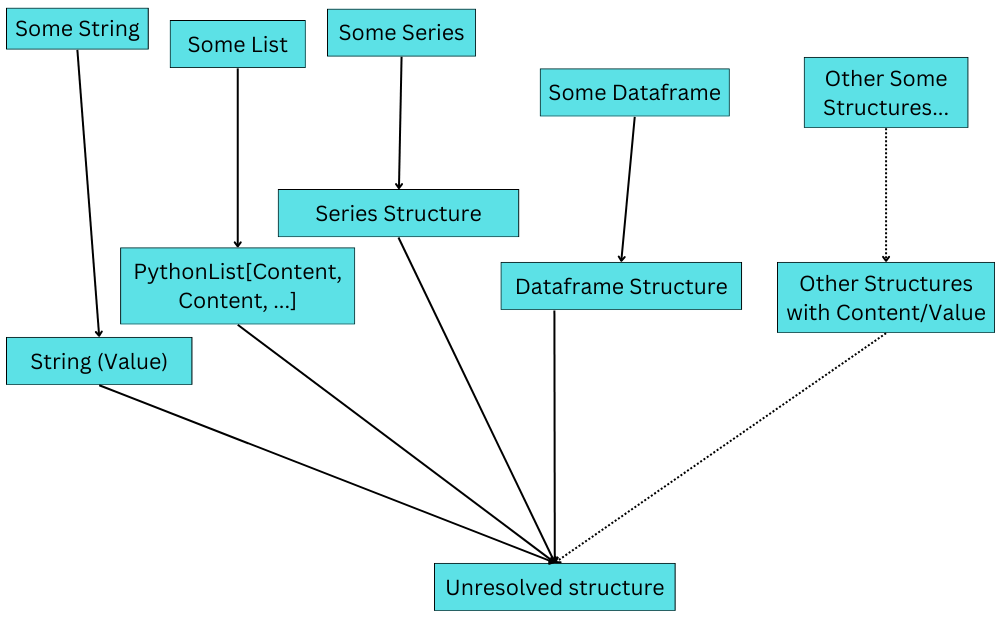
\includegraphics[scale=0.5]{img/Hierarchy}
\end{figure}

To satisfy the definition of a Lattice, every pair of elements must have a supremum and infimum.
It can be seen from the Figure~\ref{fig:abstract_hierarchy} that the infimum exists.
For two different values of the same type \verb|String("first")| and \verb|String("second")|, the infimum is
\verb|SomeString|.
For the two different types \verb|String("str")| and \verb(Int(7))|, the infimum is \verb|UnresolvedStructure|.
The other cases are analogous and are left as an exercise for the reader.

However, the idea misses suprema.
For that purpose we define another structure called \verb|NondeterministicStructure|.
The supremum of two elements of the hierarchy \verb|a| and \verb|b| is \verb|NondeterministicStructure(a, b)|.
The idea is also applicable recursively, so the value \\
\begin{verbatim}
NondeterministicStructure(
    NondeterministiStructure(
        SomeString,
        SomeInt
    ),
    SomeSeries
)
\end{verbatim}
is a valid element of the hierarchy.
The idea is shown in the Figure~\ref{fig:nondeterministic_structure}
With this idea, the hierarchy is finally a Lattice.
Note that it is not a Complete Lattice as the whole hierarchy does not have a supremum.

\begin{figure}[H]
    \caption{Nondeterministic structure}
    \label{fig:nondeterministic_structure}
    \centering
    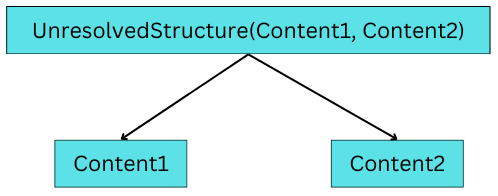
\includegraphics[scale=0.5]{img/unresolved_structure}
\end{figure}

The Nondeterministic Structure will mostly occur when there is a branching (e.g.~an if-statement) in the program, and we are not
able to resolve which branch we should go.
So the Nondeterministic Structure is a substitute that we need to use since we do not use the power set as the abstract
lattice anymore.


\section{Limitations}

The presented framework has some limitations that are important to discuss.
First, remembering just a Dataframe Structure prevents us from doing operations, that have the resulting Dataframe
Structure dependent on the values in a Dataframe.
Example of such operation can be the pivot operation.
The result of a pivot operation has columns named after values from a selected column.
But we do not know these values, since we only remember the Dataframe Structure.
Another example of an operation, that we are unable to resolve the resulting Dataframe of is a transpose.
The transpose function flips the whole dataframe along the diagonal (like with matrices), so the columns of the result
will be the rows of the original Dataframe and the column names of the result will be the index values of the original.
But, again, we do not know the index values.
In such situation there is no other option then just returning Some Dataframe.

Another possible problem can be an unknown value propagation, meaning that when there is a value with any uncertainty
(e.g.\ Nondeterministic Structure or Some value), using this value in an operation will in most cases lead to an
operation result with an uncertainty as well.

\section*{Summary}
\addcontentsline{toc}{section}{Summary}

\xxx{TODO :)}
\chapter{Pandalyzer}

\section{Functionality}

\section{Architecture}

\section{User documentation}

\section*{Summary}
\addcontentsline{toc}{section}{Summary}
\chapter{Evaluation of solution}\label{ch:evaluation-of-solution}

This chapter is dedicated to the evaluation of the implementation presented in the previous chapter.
We design a set of realistic case studies for Pandas and evaluate the quality of analysis of the proposed solution.
We do not define any specific metrics for the evaluation since it is cumbersome to do it rigidly.
We rather look at the analysis from the more intuitive perspective and discuss which useful analysis features are
provided and which could be missing.

\section{Case Studies}

Each case study contains:
\begin{itemize}
    \item Explanation of the case
    \item An example code in Python
    \item Description of possible mistakes
    \item The output of the analyzer in the good case and in the case with mistakes
\end{itemize}

\paragraph{Case Study \#1:} Multiple operations, multiple Dataframes, no uncertainty  \\

The purpose of the first case study is to show the capabilities of Pandalyzer in a deterministic environment when
the Pandalyzer has all the information it needs for the analysis and there is no uncertainty.
There are, however, many different operations with multiple Dataframes.
We show that Pandalyzer is able to check input for all these operations and determine their output.

In this case study we work with a data from sport competitions agency.
We get a csv file with competitions that they organized.
We also get a csv file with all attendees of these competitions.
Last file contains information about the number of points that an attendee got from a specific competition.

The \verb|config.toml| (and the csv column structure) is shown in the listing~\ref{lst:cs1_config}

\begin{lstlisting}[caption=config.toml of the first case study, label={lst:cs1_config}, captionpos=b]
[attendees.csv]
name = "string"
surname = "string"
age = "int"

[matches.csv]
id = "int"
name = "string"

[scores.csv]
name_surname = "string"
match_id = "int"
score = "int"
\end{lstlisting}

Our goal is to create a csv file called top\_two\_per\_age.csv that contains the top two attendees per age per sport match
together with the sport match name.

The listing~\ref{lst:cs1_code} shows how that could be implemented in Pandas.

\begin{lstlisting}[caption=Solution of the first case study in Pandas, label={lst:cs1_code}, captionpos=b, numbers=left]
import pandas as pd

attendees_df = pd.read_csv("attendees.csv")
matches_df = pd.read_csv("matches.csv") \
    .rename(columns={"name": "match_name"})
scores_df = pd.read_csv("scores.csv")

attendees_df["name_surname"] = \
    attendees_df["name"] + "_" + attendees_df["surname"]
attendees_df = attendees_df.drop(columns=["name", "surname"])

scores_with_match_name_df = scores_df \
    .merge(matches_df, left_on="match_id", right_on="id") \
    .drop(columns="id")

scores_with_age_df = pd.merge(
    scores_with_match_name_df, attendees_df, on="name_surname"
)

top_two_per_age_df = scores_with_age_df \
    .sort_values("age") \
    .groupby(["age", "match_name"]) \
    .head(2) \
    .drop(columns=["match_id"])

top_two_per_age_df.to_csv("top_two_per_age.csv")
\end{lstlisting}

Let us break down the code in the listing~\ref{lst:cs1_code}.
We first read all the CSV files and store the data to Pandas Dataframes.
We also rename the \verb|name| column in \verb|matches_df| to \verb|match_name| so that the name of the column makes
sense later when it is merged with other Dataframes.
This is the first tricky part, since from now on we have to remember that the \verb|matches_df| does not contain a name
column but rather a \verb|match_name| column.
Then, since \verb|attendees_df| contains \verb|name| and \verb|surname| columns and the \verb|scores_df| contains
\verb|name_surname|, we also have to create a new column \verb|name_surname| in the \verb|attendees_df| and drop the
old columns (\verb|name| and \verb|surname|).
The next two operations merge the three Dataframes to a \verb|scores_with_age_df|.
We can notice that it is now already hard to keep track of the structure of the Dataframes.
Then the Dataframe is sorted by \verb|age|, grouped by \verb|age| and \verb|match_name| and the first two items from each group are selected.
Also, we drop the \verb|match_id| since we do not need it in the final data.
The resulting Dataframe is stored to a CSV file called \verb|top_two_per_age.csv|.

This case study shows two ideas.
First, it is hard to keep track of everything what is happening with the Dataframes, and it is easy to do a mistake
e.g.~access already non-existent column, misspell the column name or incorrectly specify the arguments of a pandas function.
Second, the scenario where we are able to deterministically derive the structure of the resulting data (e.g.~it does not
depend on any user input or other sources of uncertainty) can be a very realistic scenario. % todo is this clear enough?

What we want from the Pandalyzer in this case is to give us the structure of the \verb|top_two_per_age.csv| file
and warn us in case that we do any of the mistakes mentioned.
The listing~\ref{lst:cs1_pandalyzer_normal} shows the output of the Pandalyzer given the input shown in the
listing~\ref{lst:cs1_code} and the configuration shown in the listing~\ref{lst:cs1_config}.

\begin{lstlisting}[caption=Output of Pandalyzer on the first case study, label={lst:cs1_pandalyzer_normal}, captionpos=b]
Summary of analysis: OK
Global data structures (7):
pd: PandasImport
attendees_df: DataFrame(columns={age=IntType,
    name_surname=StringType})
matches_df: DataFrame(columns={id=IntType,
    match_name=StringType})
scores_df: DataFrame(columns={name_surname=StringType,
    match_id=IntType, score=IntType})
scores_with_match_name_df: DataFrame(columns={
    name_surname=StringType, match_id=IntType,
    score=IntType, match_name=StringType})
scores_with_age_df: DataFrame(columns={name_surname=StringType,
    match_id=IntType, score=IntType,
    match_name=StringType, age=IntType})
top_two_per_age_df: DataFrame(columns={name_surname=StringType,
    score=IntType, match_name=StringType, age=IntType})

Warnings (0):

Errors (0):

Output files (1):
File top_two_per_age.csv:
    name_surname : StringType
    score : IntType
    match_name : StringType
    age : IntType
\end{lstlisting}

The first line tells us that the no mistake was spotted in the analyzed code (otherwise there would be \verb|NOT OK|).
Then, the analyzer tells us all variables that are in the global scope when the analysis ended.
We can see all the Dataframes with their structure.
Next, we can see that the lists of Warnings and Errors are empty.
Finally, there is the \verb|Output files| summary with the \verb|top_two_per_age.csv| file structure.
The analyzer is able to tell us what columns the file contains as well as what are their types.

Now we show what happens when we do some mistake in the code.

The listing~\ref{lst:cs1_misspelled_column} shows the changed line 5 (\verb|neme| instead of \verb|name|) in the code as
well as the analysis output.

\begin{lstlisting}[caption=Misspelled column on rename function and analysis output, label={lst:cs1_misspelled_column}, captionpos=b]
    .rename(columns={"neme": "match_name"})

Summary of analysis: NOT OK
Global data structures (7):
pd: PandasImport
attendees_df: DataFrame(columns={age=IntType,
    name_surname=StringType})
matches_df: UnresolvedStructure(reason=The values
    [neme] do not exist in the dataframe)
scores_df: DataFrame(columns={name_surname=StringType,
    match_id=IntType, score=IntType})
scores_with_match_name_df: UnresolvedStructure(
    reason=Incorrect right argument to merge)
scores_with_age_df: UnresolvedStructure(reason=
    Incorrect left argument to merge)
top_two_per_age_df: UnresolvedStructure(reason=
    the attribute sort_values of UnresolvedStructure
    does not exist)

Warnings (0):

Errors (5):
0: Assign from line 4 to line 5 columns 0 - 44:
    The columns [neme] do not exist in the dataframe
1: Assign from line 12 to line 14 columns 0 - 23:
    Incorrect right argument to merge
2: Assign from line 16 to line 18 columns 0 - 1:
    Incorrect left argument to merge
3: Assign from line 20 to line 24 columns 0 - 31:
    the attribute sort_values of UnresolvedStructure
    does not exist
4: ExpressionStatement on line 26 columns 0 - 48:
    the attribute to_csv of UnresolvedStructure does not exist

Output files (0):
\end{lstlisting}

Now we can see that the result of the analysis is \verb|NOT OK|.
There are five errors in the Errors list.
The first error tells us that in the statement on lines 4--5 there is a statement where we are trying to access column
\verb|neme| that does not exist in the Dataframe.
This is enough for us to spot and fix the mistake in the code.
Other errors are in this case just consequences of the first error.

Other mistake that we can do is to specify an incorrect argument to a Pandas function.
The listing~\ref{lst:cs1_incorrect_argument} shows the changed part of the code on the line 13 (\verb|left_or| instead of
\verb|left_on|) and the analysis output.
Note that only important parts of the analysis output are shown.

\begin{lstlisting}[caption=Incorrectly specified argument and analysis output, label={lst:cs1_incorrect_argument}, captionpos=b]
    .merge(matches_df, left_or="match_id", right_on="id") \

Summary of analysis: NOT OK
/* snip */
Errors (4):
0: Assign from line 12 to line 14 columns 0 - 23:
    Got unexpected keyword arguments [left_or]
/* snip */
\end{lstlisting}

The result of the analysis is \verb|NOT OK| as expected and there is an error saying that there was an unexpected
keyword argument \verb|left_or| on the lines 12--14.


\paragraph{Case Study \#2:} Uncertainty from the user, multiple possible values \\

Next case study shows how the Pandalyzer behaves when there is some uncertainty such as an input from the user.
It also proves that the Pandalyzer is able to handle non-trivial control flow such as if-statements, functions and
early returns.

The code for this case study can be seen in the listing~\ref{lst:cs2_code}.

\begin{lstlisting}[caption=Code of the second case study in Pandas, label={lst:cs2_code}, captionpos=b]
import pandas as pd


def get_country_dataframe(country):
    if country == "Germany":
        return pd.read_csv("de.csv")
    elif country == "Austria":
        return pd.read_csv("au.csv")
    else:
        return pd.read_csv("world.csv")


def get_dataframe_from_user():
    country = input("Select a country: ")
    return get_country_dataframe(country)


user_df = get_dataframe_from_user()
user_df[["germany_specific_column"]].to_csv("output.csv")
\end{lstlisting}

And the configuration file is shown in the listing~\ref{lst:cs2_config}.

\begin{lstlisting}[caption=config.toml file for the second case study, label={lst:cs2_config}, captionpos=b]
[de.csv]
germany_specific_column = "string"
common_column = "int"

[au.csv]
common_column = "int"

[world.csv]
common_column = "int"
\end{lstlisting}

There are two functions.
The first (\verb|get_country_dataframe|) returns the Dataframe for the specified country or the Dataframe for the whole
world if the country is not known.
The second function (\verb|get_dataframe_from_user|) gets the country from the user and returns the result of
\verb|get_country_dataframe| function.
However, we do not know the result of the \verb|input| function, so we are not able to resolve which Dataframe will
be returned.
Moreover, we are trying to access the column \verb|germany_specific_column| which exists only if the user inputs
the value \verb|Germany|.
So the program can (but does not have to) crash.

The listing~\ref{lst:cs2_analysis_output} shows the output of the Pandalyzer given the input from the
listing~\ref{lst:cs2_code} and the configuration file from listing~\ref{lst:cs2_config}.

\begin{lstlisting}[caption=Analysis output of the second case study, label={lst:cs2_analysis_output}, captionpos=b]
Summary of analysis: OK
/* snip */
Warnings (6):
0: Assign on line 14 columns 4 - 41:
    Unable to resolve result of input
1: IfStatement from line 5 to line 10 columns 4 - 39:
    Unable to check unknown strings on equality
2: IfStatement from line 5 to line 10 columns 4 - 39:
    Unable to recognize the bool value in the
    if statement test - branching.
3: IfStatement from line 7 to line 10 columns 4 - 39:
    Unable to check unknown strings on equality
4: IfStatement from line 7 to line 10 columns 4 - 39:
    Unable to recognize the bool value in the
    if statement test - branching.
5: ExpressionStatement on line 19 columns 0 - 57:
    Second branch of execution failed with reason:
        Both execution branches failed.
        Branch1:
            The keys [germany_specific_column] do not
            exist in the dataframe,
        Branch2:
            The keys [germany_specific_column] do not
            exist in the dataframe

Errors (0):

Output files (1):
File output.csv:
    germany_specific_column : StringType

\end{lstlisting}

This time the output is more complicated.
The result of the analysis is \verb|OK| since the fact that some branch can fail does not mean that the whole program is
incorrect.
However, there are five warnings.
The first warnings is related to the \verb|input| function itself.
It just tells the user that an uncertainty occurred.
The next four warnings are related to the fact that we are trying to compare a string with unknown value and then
trying to branch based on the result.
The Pandalyzer tells us that it is branching (executing both branches) in that case.
The last warning is the most important.
It is less readable, but that is just because the problem is complicated.
It tells us that one of the branches failed, and it gives us the reason.
The reason is that both branches in the second branch failed, and it gives us the reasons.
The Pandalyzer also tells us that there is an output file.
It corresponds to the branch of execution in which the user input was \verb|Germany|.


\paragraph{Case Study \#3:} Regex config, column compatibility \\

Now we have a set of files 30\_04\_2024\_production.csv and 31\_04\_2024\_production.csv that contain per-hour production
of some factory on a given day.
We are interested in hours when the production was lower than 400 items.
This time we use the regex feature of our configuration.
The \verb|config.toml| file will be as shown in listing~\ref{lst:cs3_config}.

\begin{lstlisting}[caption=config.toml of the second case study, label={lst:cs3_config}, captionpos=b]
r[^\d{2}_\d{2}_\d{4}_production\.csv$]
hour = "int"
production = "int"
note = "string"
\end{lstlisting}

The record in the \verb|config.toml| file says that all the csv files with the name dd\_mm\_yyyy\_production.csv have the
specified columns structure.
The regex feature is useful for large amount of same-structured files with similar names (different only in date,
number etc.).

The code solving this problem can be seen in Listing~\ref{lst:cs3_code}

\begin{lstlisting}[caption=Solution of the third case study in Pandas, label={lst:cs3_code}, captionpos=b, numbers=left]
import pandas as pd

tuesday_df = pd.read_csv("30_04_2024_production.csv")
wednesday_df = pd.read_csv("31_04_2024_production.csv")

tuesday_df["day"] = 30
wednesday_df["day"] = 31

agg_df = pd.concat([tuesday_df, wednesday_df])

low_production_df = agg_df[agg_df["production"] < 400]

low_production_df.to_csv("aggregate_production.csv")
\end{lstlisting}

The output of the Pandalyzer given the input from listing~\ref{lst:cs3_code} and the configuration from
listing~\ref{lst:cs3_config} is shown in the listing~\ref{lst:cs3_analysis_output}

\begin{lstlisting}[caption=Analysis output of the third case study, label={lst:cs3_analysis_output}, captionpos=b]
Summary of analysis: OK
Global data structures (5):
pd: PandasImport
tuesday_df: DataFrame(columns={hour=IntType,
    production=IntType, note=StringType, day=IntType})
wednesday_df: DataFrame(columns={hour=IntType,
    production=IntType, note=StringType, day=IntType})
agg_df: DataFrame(columns={hour=IntType,
    production=IntType, note=StringType, day=IntType})
low_production_df: DataFrame(columns={hour=IntType,
    production=IntType, note=StringType, day=IntType})

Warnings (0):

Errors (0):

Output files (1):
File aggregate_production.csv:
    hour : IntType
    production : IntType
    note : StringType
    day : IntType
\end{lstlisting}

As expected, the result of the analysis is \verb|OK| and the lists of Warnings and Errors are empty.
There is one output file \verb|aggregate_production.csv| with the correct structure.
The Pandalyzer was also able to match the input filenames with the regex in the configuration file.
An important part of the analysis is the \verb|concat| function.
The result of the function has the same structure as the inputs, but it requires the inputs to have the same structure.
Let us see what the analyzer outputs if we change the structure of one of the Dataframes.
The listing~\ref{lst:cs3_incompatible_concat} shows the changed line TODO\ldots

\begin{lstlisting}[caption=Incompatible Dataframes to concat operation and analysis output, label={lst:cs3_incompatible_concat}, captionpos=b]
tuesday_df["another_column"] = 30

Summary of analysis: NOT OK
/* snip */
Errors (3):
0: Assign on line 9 columns 0 - 46:
    All dataframes to be concatenated must have
    the same column structure
/* snip */
\end{lstlisting}

The Pandalyzer detected the mistake.
The result of the analysis is \verb|NOT OK| and there is an error saying that all Dataframes ot be concatenated must
have the same structure.


\paragraph{Case Study \#4:} High uncertainty, user input \\

The fourth case study again focuses on the uncertainty, but it shows different use cases of uncertainty than the second
case study.

\paragraph{Case Study \#5:} Group by, aggregations \\

In the last case study, we go over some use cases of the group by operation and the associated aggregations.
Let us have the following configuration file (shown in listing~\ref{lst:cs5_config}):

\begin{lstlisting}[caption=config.toml file for the fifth case study, label={lst:cs5_config}, captionpos=b]
[all_strings.csv]
str1 = "string"
str2 = "string"
str3 = "string"

[first_string.csv]
col1 = "string"
col2 = "int"
col3 = "int"

[first_int.csv]
col1 = "int"
col2 = "string"
col3 = "string"

[all_different.csv]
int_col = "int"
str_col = "string"
bool_col = "bool"
\end{lstlisting}

The source code for the case study can be seen in the listing~\ref{lst:cs5_code}.

\begin{lstlisting}[caption=Code of the fifth case study in Pandas, label={lst:cs5_code}, captionpos=b, numbers=left]
import pandas as pd

all_strings_df = pd.read_csv("all_strings.csv")
first_string_df = pd.read_csv("first_string.csv")
first_int_df = pd.read_csv("first_int.csv")
all_different_df = pd.read_csv("all_different.csv")

pass_df1 = first_string_df.groupby("col1").mean()
fail_df1 = first_string_df.groupby("col2").mean()

pass_df2 = all_strings_df.groupby("str1").count()["str2"] + 3
fail_df2 = all_strings_df.groupby("str1").count()["str2"] + "hi"

pass_df3 = all_different_df.groupby("bool_col").sum()
fail_df3 = all_different_df.groupby("str_col").sum()

pass_df4 = first_int_df.groupby(["col2", "col3"]).mean()
fail_df4 = first_int_df.groupby("col3").mean()
\end{lstlisting}

The code reads all four CSV files defined and stores them in the Dataframes.
Then, there are four pairs group by operations followed by aggregations.
Every pair has one operation that passes and one that fails.

The first pair applies the \verb|mean| function on the \verb|first_string_df| grouped by \verb|col1| and by \verb|col2|.
However, only the first option passes.
The reason is that the mean function is applied to all columns that we did not group by.
So in the second case it is also the \verb|col1| column which is string.
But the mean function cannot be applied on a string column.

The second pair shows the usage of \verb|count| function on the \verb|all_strings_df| grouped by \verb|str1|.
The count should return an int column for all columns that we did not group by.
So summing some of the columns with a number should pass and summing it with string should fail.

In the third pair we apply the sum function to non-grouped columns.
In the first case it is \verb|str_col| and \verb|int_col|, which can be summed.
In the second case it is \verb|int_col| and \verb|bool_col|.
The second case will actually \textbf{not} fail this time.
But summing of bool column is usually something that we do not want, so we should consider it an error.

The last (fourth) case again computes a mean.
This time, the first case will not fail, since the only column we apply mean on is \verb|col1| which is an int column.
The second case will fail, since we apply the mean on both the \verb|col1| and \verb|col2|, but the \verb|col2| is
a string column which we cannot apply mean on.

The listing~\ref{lst:cs5_analysis_output} shows the output of the Pandalyzer on the code in the listing~\ref{lst:cs5_code}
and the configuration in the listing~\ref{lst:cs5_config}.

\begin{lstlisting}[caption=Analysis output of the fifth case study, label={lst:cs5_analysis_output}, captionpos=b]
Summary of analysis: NOT OK
\* snip *\
Warnings (0):

Errors (4):
0: Assign on line 9 columns 0 - 49:
    Cannot apply mean on the columns: col1 of type StringType,
1: Assign on line 12 columns 0 - 67:
    Cannot sum a series of type IntType with PythonString
2: Assign on line 15 columns 0 - 52:
    Cannot apply sum on the columns: bool_col of type BoolType,
3: Assign on line 18 columns 0 - 46:
    Cannot apply mean on the columns: col2 of type StringType,

Output files (0):
\end{lstlisting}

The analysis shows exactly what we said.
There are four errors, each explaining one of the mistakes discussed.

\section*{Summary}
\addcontentsline{toc}{section}{Summary}


\chapter*{Conclusion}
\addcontentsline{toc}{chapter}{Conclusion}

The aim of this thesis was to design and implement a code-analysis tool for the Pandas library that would be capable of
checking common kinds of errors such as accesses to misspelled or non-existent columns.
The resulting system should have been evaluated through a set of realistic case studies.
Let us recap and summarize to what extent we did that.

We first defined a framework for the Abstract Interpretation analysis of the Dataframe and Series type and then expanded it
to other types such as strings, numbers, lists, etc.
Then we used the framework to implement the Pandalyzer.
The Pandalyzer is a code-analysis tool that uses Abstract Interpretation to interpret Python code with Pandas
library.
The Pandalyzer is capable of detecting errors such as access to non-existent column, operation on incompatible types,
incorrect function arguments, operations leading to an incorrect state.
It also reports the structure of the output CSV files and is able to accept information about the structure of the input CSV files.
The Pandalyzer is able to work with some amount of uncertainty generated from the user input.
The supported functions include merge, groupby, drop, rename, read\_csv, to\_csv, concat, Dataframe creation,
Series creation, the subscript operator in both get and set contexts and vectorized sums and products, aggregation function
such as mean, sum, first, last, count or head.
As shown in the case studies in the chapter~\ref{ch:evaluation-of-solution}, this set of functions already gives
the user enough flexibility to do many various data manipulation tasks.
Moreover, the Pandalyzer is highly extensible, so implementing support for other Pandas functions is possible.

On the other hand, the Pandalyzer has some limitations.
It now only supports a subset of Python language so the analyzer will not be able to proceed with the analysis when
it encounters unknown Python construct.
However, it is planned in the Future Work~\ref{sec:future-work} to add support for the rest of the Python language.

\section*{Related Work}
\addcontentsline{toc}{section}{Related Work}

The idea to use Abstract Interpretation to analyze programs working with Dataframes was already proposed by~Yungyu~Zhuang
and~Ming-Yang~Lu~\cite{Zhuang:2022:TypeChecking}.
They also created a proof of concept implementation named PDChecker.
However, PDChecker does not have as many checks, does not report output CSV files (via to\_csv() function) and
does not allow for interpreting multiple branches of if-statements and other sources of non-determinism.

Another related subject are the type hints~\cite{python_typing} in Python language.
The language itself does not enforce any typing rules, but we can put type annotations in the code and analyzers
integrated in the IDE can warn us in case that the types do not match.
Unfortunately, this is not useful for our case, since the type annotations are only able to express that
(for example) the function returns a Pandas Dataframe, not a Pandas Dataframe with a specific column structure.

The Types for Tables~\cite{types_for_tables} article defines the Table API - the definition of a table and operations on
a table similarly as we did it in the chapter~\ref{ch:putting-it-all-together}.


\section*{Future Work}\label{sec:future-work}
\addcontentsline{toc}{section}{Future Work}

There is a lot of plans ahead of us regarding the implementation.
In the future, we would like to support more Pandas operations since Pandas is a large library with many useful
operations.
We would also like to add support for working with Indexes on Dataframes and Series.
The Pandalyzer so far supports a limited subset of Python language constructs.
We chose the most useful language constructs for the data manipulation.
However, the plan for the future is to add support for other Python constructs such as Lambdas, Match statements,
For-loops or Classes.
As of now, Pandalyzer is only able to analyze one module, so extending it to be able to analyze multiple modules together
could be also a useful extension.

The Pandalyzer tool could be also extended for other related Python libraries.
A good example is the numpy library for working with vectors, matrices etc.
The abstraction could be defined as the dimensions of the vectors and matrices.
Another good example of a library worth including to the Pandalyzer is the matplotlib library for data visualization.
We could support reporting of what visualizations would be displayed to the user.
This could be implemented in a similar way as the analysis of the to\_csv function in Pandas.

Another field where the Pandalyzer could be extended is its integration to the IDEs such as PyCharm or VS Code.
This could be done using the Language Server Protocol.

%%% Bibliography
%%% Bibliography (literature used as a source)
%%%
%%% We employ biblatex to construct the bibliography. It processes
%%% citations in the text (e.g., the \cite{...} macro) and looks up
%%% relevant entries in the bibliography.bib file.
%%%
%%% See also biblatex settings in thesis.tex.

%%% Generate the bibliography. Beware that if you cited no works,
%%% the empty list will be omitted completely.

% We let bibliography items stick out of the right margin a little
\def\bibfont{\hfuzz=2pt}

\printbibliography[heading=bibintoc]

%%% If case you prefer to write the bibliography manually (without biblatex),
%%% you can use the following. Please follow the ISO 690 standard and
%%% citation conventions of your field of research.

% \begin{thebibliography}{99}
%
% \bibitem{lamport94}
%   {\sc Lamport,} Leslie.
%   \emph{\LaTeX: A Document Preparation System}.
%   2nd edition.
%   Massachusetts: Addison Wesley, 1994.
%   ISBN 0-201-52983-1.
%
% \end{thebibliography}


%%% Figures used in the thesis (consider if this is needed)
\listoffigures

%%% Tables used in the thesis (consider if this is needed)
%%% In mathematical theses, it could be better to move the list of tables to the beginning of the thesis.
\listoftables

%%% Abbreviations used in the thesis, if any, including their explanation
%%% In mathematical theses, it could be better to move the list of abbreviations to the beginning of the thesis.
\chapwithtoc{List of Abbreviations}

\textbf{Poset} - Partially ordered set

\textbf{AST} - Abstract syntax tree

%%% Doctoral theses must contain a list of author's publications
\ifx\ThesisType\TypePhD
\chapwithtoc{List of Publications}
\fi

%%% Attachments to the thesis, if any. Each attachment must be referred to
%%% at least once from the text of the thesis. Attachments are numbered.
%%%
%%% The printed version should preferably contain attachments, which can be
%%% read (additional tables and charts, supplementary text, examples of
%%% program output, etc.). The electronic version is more suited for attachments
%%% which will likely be used in an electronic form rather than read (program
%%% source code, data files, interactive charts, etc.). Electronic attachments
%%% should be uploaded to SIS. Allowed file formats are specified in provision
%%% of the rector no. 72/2017. Exceptions can be approved by faculty's coordinator.
\appendix

\chapter{User documentation}\label{ch:user-documentation}


\section{Building from source}

To build the Pandalyzer from sources, follow the steps below:
\begin{enumerate}
    \item Ensure that you have Java(version 21.0.1 or higher), Git and Python 3.x installed.
    \item Clone the Pandalyzer repository:

    \verb|git clone https://github.com/Hrubian/Pandalyzer.git|
    \item Navigate to the root folder of the repository:

    \verb|cd Pandalyzer|
    \item Run the Gradle bootstrap script:

    \verb|./gradlew build| or \verb|./gradlew.bat build| on Windows
\end{enumerate}

\section{Running the tool}

The build generates a \verb|./build/| folder.
There is also \verb|./build/distributions/Pandalyzer.tar| and \verb|./build/distributions/Pandalyzer.zip| archives.
Unpack one of them (depending on what tools you are provided with) and run the \verb|Pandalyzer| (or
\verb|Pandalyzer.bat|) script in the \verb|bin| folder.
The program accepts the following command-line arguments:
\begin{itemize}
    \item -h, --help - Prints usage information and exits
    \item -i, --input - The input python script to analyze \textbf{(mandatory)}
    \item -o, --output - The output file to store the analysis result to (standard output by default)
    \item -c, --config - The configuration file to read the file structures from (config.toml by default)
    \item -f, --format - The format of the analysis output, possible options: hr (human-readable), json (hr by default), csv
\end{itemize}

%\chapter{Attachments}
%
%\section{First Attachment}

\end{document}
